\subsection{Методы обнаружения аномалий на основе нейронных сетей}

Методы обнаружения аномалий на основе нейронных сетей в настоящее время являются одним из наиболее перспективных направлений анализа поведения информационных систем. Их основное преимущество заключается в способности автоматически извлекать скрытые закономерности из данных, учитывать нелинейные зависимости и моделировать сложные временные или структурные связи, которые трудно формализовать с помощью правил или классических алгоритмов машинного обучения.

К числу наиболее распространённых нейросетевых подходов к обнаружению аномалий относятся:

\begin{itemize}
    \item \textbf{Рекуррентные нейронные сети (Recurrent Neural Networks, RNN)} — используются для анализа последовательных данных и временных зависимостей;
    \item \textbf{Сети с долгой краткосрочной памятью (Long Short-Term Memory, LSTM)} — разновидность рекуррентных сетей, лучше сохраняющая долгосрочный контекст;
    \item \textbf{Автоэнкодеры (Autoencoders, AE)} — используются для моделирования нормального поведения и выявления аномалий по ошибке реконструкции.
\end{itemize}

\subsubsection{Рекуррентные нейронные сети (RNN)}

\textbf{Рекуррентные нейронные сети (RNN)} — это класс нейронных сетей, предназначенных для обработки последовательных данных с учётом временных зависимостей. RNN содержат рекуррентные связи, позволяющие скрытому состоянию на каждом временном шаге сохранять информацию о предыдущих входах. Это создаёт эффект памяти и контекста \cite{RNN}. Благодаря этому RNN подходят для задач, где важны порядок элементов и история наблюдений, например для прогнозирования временных рядов, анализа текста и речи \cite{RNNs_and_LSTMs}.

На рисунке~\ref{fig:RNN_arch} показана архитектура RNN. На каждом временном шаге $t$ входной вектор $x_t$ преобразуется с помощью матриц весов и функции активации в скрытое состояние $h_t$, которое затем используется для получения выхода $y_t$. Ключевое отличие RNN заключается в том, что при вычислении текущего состояния учитывается предыдущее скрытое состояние $h_{t-1}$, что и обеспечивает механизм памяти.

\begin{figure}
    \centering
    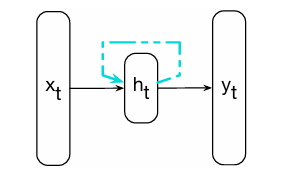
\includegraphics[scale=0.9]{inc/images/Simple-RNN-arch}
    \caption{Архитектура RNN \cite{RNNs_and_LSTMs}.}
    \label{fig:RNN_arch}
\end{figure}

RNN удобно представлять как сеть с прямой связью, «развернутую» по времени, где каждый узел скрытого слоя принимает на вход ранее вычисленное состояние. Такой подход показан на рисунке~\ref{fig:RNN_forward_inference}.

\begin{figure}
    \centering
    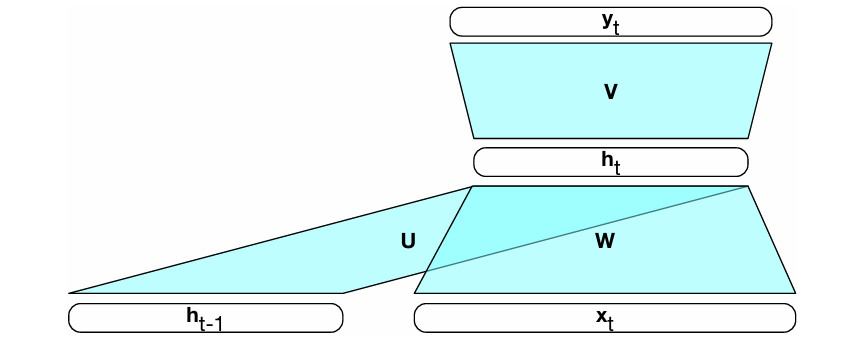
\includegraphics[scale=0.6]{inc/images/Simple-RNN-arch illustration feedforward}
    \caption{Архитектура RNN, представленная как сеть с прямой связью \cite{RNNs_and_LSTMs}.}
    \label{fig:RNN_forward_inference}
\end{figure}

Прямой проход RNN описывается следующими уравнениями. Скрытое состояние $h_t$ на шаге $t$ вычисляется по рекуррентному правилу, представленному в формуле~\ref{rnn_h_t}.

\begin{equation}\label{rnn_h_t}
    h_t = g(W x_t + U h_{t-1} + b_h),
\end{equation}

где $W$ — матрица весов для входа, $U$ — матрица рекуррентных весов, $b_h$ — вектор смещений, а $g(\cdot)$ — нелинейная функция активации, например $\tanh$ или ReLU. Выход сети \(y_t\) на шаге \(t\) определяется выражением, приведённым в формуле~\ref{rnn_y_t}.

\begin{equation}\label{rnn_y_t}
    y_t = f(V h_t + b_y),
\end{equation}

где $V$ — матрица весов между скрытым и выходным слоями, $b_y$ — вектор смещений выходного слоя, а $f(\cdot)$ — функция активации, часто используемая для нормализации выходов, например \texttt{softmax} для задач классификации.
Процедура вычисления выполняется последовательно по временным шагам: сначала $h_1$, затем $h_2$ и так далее до $h_T$. Таким образом, результат зависит от порядка элементов входной последовательности.

\textbf{Преимущества RNN:}
\begin{enumerate}
    \item Способность моделировать последовательные и временные зависимости между входными данными.
    \item Эффективное использование параметров: одни и те же веса применяются на всех временных шагах.
    \item Обработка входов переменной длины.
    \item Возможность онлайн-обучения на новых данных без полной перестройки модели.
\end{enumerate}

\textbf{Недостатки RNN:}
\begin{enumerate}
    \item Проблемы затухающих и взрывающих градиентов при обучении, затрудняющие захват долгосрочных зависимостей.
    \item Ограниченная способность к долгосрочной памяти в классических архитектурах.
    \item Последовательная природа вычислений затрудняет параллельное обучение и увеличивает вычислительную нагрузку.
\end{enumerate}

\subsubsection{Сети с долгой краткосрочной памятью (LSTM)}

\textbf{Long Short-Term Memory (LSTM)} — это разновидность рекуррентных нейронных сетей (RNN), разработанная для решения проблемы затухающих и взрывающих градиентов, характерной для классических RNN. Благодаря этому LSTM эффективно моделируют долгосрочные зависимости в последовательных данных, что сделало их одной из наиболее популярных архитектур для анализа временных рядов, текста и других последовательностей \cite{LSTM}.

Основная идея LSTM заключается в управлении потоком информации во времени с помощью механизмов ворот (gates). Ворота позволяют сети решать, какую информацию сохранить, обновить или забыть. Для этого в архитектуру LSTM добавляется вектор состояния ячейки (cell state), который играет роль долговременной памяти.

Каждый LSTM-блок содержит три основных типа ворот:

\begin{enumerate}
    \item \textbf{Ворота забывания (Forget gate)} — определяют, какая часть информации из предыдущего состояния $c_{t-1}$ должна быть сохранена или удалена;
    \item \textbf{Входные ворота (Input gate)} — контролируют добавление новой информации в состояние ячейки;
    \item \textbf{Выходные ворота (Output gate)} — определяют, какая часть обновлённого состояния $c_t$ передается в скрытое состояние $h_t$.
\end{enumerate}

\textbf{Ворота забывания} вычисляют взвешенную сумму скрытого слоя предыдущего состояния $h_{t-1}$ и текущего входного вектора $x_t$ и пропускают её через сигмоидную функцию (формула ~\ref{lstm_f_t}). Эта маска $f_t$ затем поэлементно умножается (произведение Адамара) на вектор предыдущего контекста $c_{t-1}$, чтобы удалить из него информацию, которая больше не требуется (формула ~\ref{lstm_k_t}).

\begin{equation}\label{lstm_f_t}
    f_t = \sigma(U_f h_{t-1} + W_f x_t)
\end{equation}

\begin{equation}\label{lstm_k_t}
    k_t = c_{t-1} \odot f_t
\end{equation}

\textbf{Входные ворота} управляют добавлением новой информации в память. Сначала вычисляется кандидат на обновление памяти $g_t$, представляющий возможное новое содержимое контекста (формула~\ref{lstm_g_t}).

\begin{equation}\label{lstm_g_t}
    g_t = \tanh(U_g h_{t-1} + W_g x_t)
\end{equation}

Функция $\tanh(\cdot)$ ограничивает значения в диапазоне $(-1, 1)$, что повышает устойчивость обновлений. Далее вычисляется сигмоидная маска $i_t$, определяющая степень добавления новых данных в память (формула~\ref{lstm_i_t}).

\begin{equation}\label{lstm_i_t}
    i_t = \sigma(U_i h_{t-1} + W_i x_t)
\end{equation}

Эти два вектора поэлементно умножается (формула~\ref{lstm_j_t}), что формирует итоговое обновление памяти.

\begin{equation}\label{lstm_j_t}
    j_t = g_t \odot i_t
\end{equation}

Итоговое состояние ячейки вычисляется как сумма модифицированного старого состояния $k_t$ и нового добавления $j_t$ (формула~\ref{lstm_c_t}).

\begin{equation}\label{lstm_c_t}
    c_t = k_t + j_t
\end{equation}

\textbf{Выходные ворота} определяют, какая часть обновлённого контекста $c_t$ используется для формирования скрытого состояния $h_t$. Сначала вычисляется маска выхода $o_t$ (формула~\ref{lstm_o_t}).

\begin{equation}\label{lstm_o_t}
    o_t = \sigma(U_o h_{t-1} + W_o x_t)
\end{equation}

Затем скрытое состояние определяется как поэлементное произведение маски выхода $o_t$ и нелинейно преобразованного контекста (формула~\ref{lstm_h_t}).

\begin{equation}\label{lstm_h_t}
    h_t = o_t \odot \tanh(c_t)
\end{equation}

Рисунок~\ref{fig:LSTM_arch} иллюстрирует полный процесс вычислений в одном блоке LSTM. Блок принимает на вход текущее наблюдение, скрытое состояние предыдущего шага и состояние ячейки, после чего формирует обновлённые значения на выходе. Именно скрытое состояние $h_t$ используется как выход LSTM на каждом временном шаге.

\begin{figure}
    \centering
    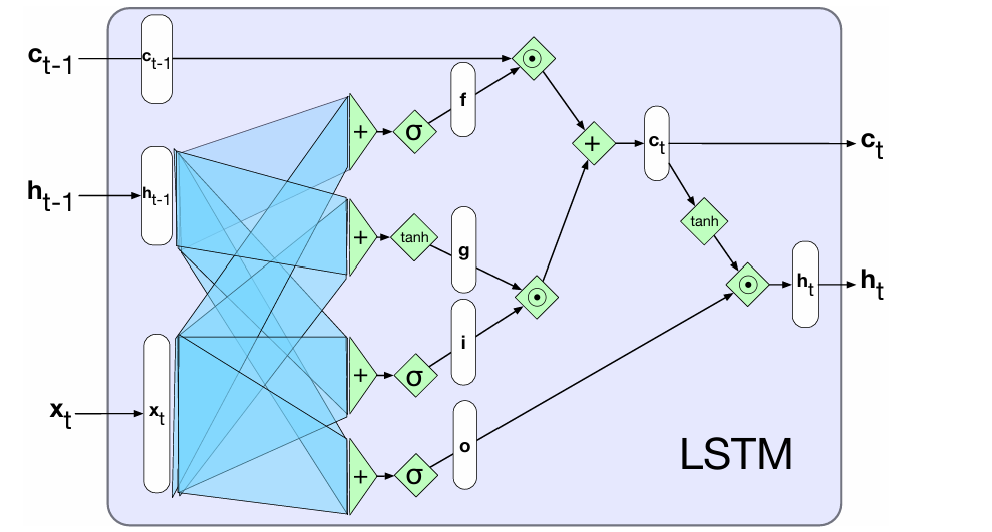
\includegraphics[scale=0.8]{inc/images/LSTM-arch}
    \caption{Архитектура LSTM \cite{RNNs_and_LSTMs}.}
    \label{fig:LSTM_arch}
\end{figure}

Архитектура LSTM естественным образом подходит для анализа метрик и логов Kubernetes-кластера, поскольку она оптимизирована для работы с последовательными и временными рядами.

\subsubsection{Автоэнкодеры}

\textbf{Автокодировщик (Autoencoder, AE)} — это нейросетевая модель, которая обучается сжимать входные данные в компактное латентное представление и восстанавливать исходные данные по этому представлению. Цель обучения состоит в минимизации ошибки восстановления, например MSE или бинарной кросс-энтропии, благодаря чему модель извлекает информативные признаки входных данных \cite{AE}.

Архитектура автокодировщика состоит из двух основных частей:

\begin{itemize}
    \item \textbf{Encoder} — преобразует входной вектор признаков $x$ в компактное скрытое представление $z$;
    \item \textbf{Decoder} — восстанавливает исходный вектор $\tilde{x}$ по скрытому представлению $z$.
\end{itemize}

На рисунке~\ref{fig:AE_arch} представлена типичная архитектура автокодировщика. Входной вектор признаков проходит через несколько полносвязных слоёв Encoder, которые последовательно уменьшают размерность представления. Центральный слой формирует латентное пространство, содержащее компактное описание входных данных. Затем Decoder восстанавливает исходный вектор признаков.

\begin{figure}
    \centering
    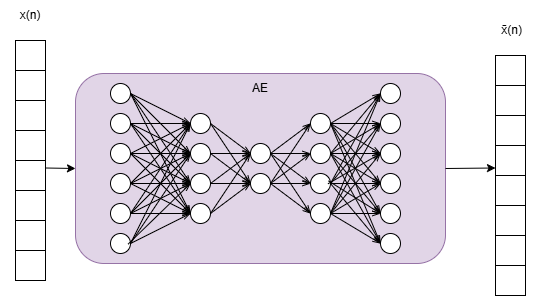
\includegraphics[scale=0.6]{inc/images/autoencoder_architecture}
    \caption{Архитектура классического Autoencoder.}
    \label{fig:AE_arch}
\end{figure}

Математически процесс кодирования описывается в формуле~\ref{eq:encoder}.

\begin{equation}\label{eq:encoder}
    z = g(W_e x + b_e)
\end{equation}

где $W_e$ — матрица весов Encoder, $b_e$ — вектор смещений, а $g(\cdot)$ — функция активации.

Процесс декодирования, описанный в формуле~\ref{eq:decoder}, восстанавливает исходный вектор признаков.

\begin{equation}\label{eq:decoder}
    \tilde{x} = f(W_d z + b_d)
\end{equation}

где $W_d$ — матрица весов Decoder, $b_d$ — вектор смещений, а $f(\cdot)$ — функция активации выходного слоя.

Таким образом, автокодировщик аппроксимирует функцию восстановления, представленную в формуле~\ref{eq:ae_mapping}.

\begin{equation}\label{eq:ae_mapping}
    \tilde{x} = f(W_d g(W_e x + b_e) + b_d)
\end{equation}